
%(BEGIN_QUESTION)
% Copyright 2006, Tony R. Kuphaldt, released under the Creative Commons Attribution License (v 1.0)
% This means you may do almost anything with this work of mine, so long as you give me proper credit

Her vises responsen til en proporsjonal+deriverende regulator på en rampende prosessvariabel (med konstant settpunkt). Beregn regulatorens proporsjonal- og derivasjonskonstanter basert på det du ser i grafen. Bestem også om regulatoren er direkte- eller reversvirkende, og marker trekkene i utgangsplotet som tilsvarer proporsjonal virkning og deriverende virkning.

$$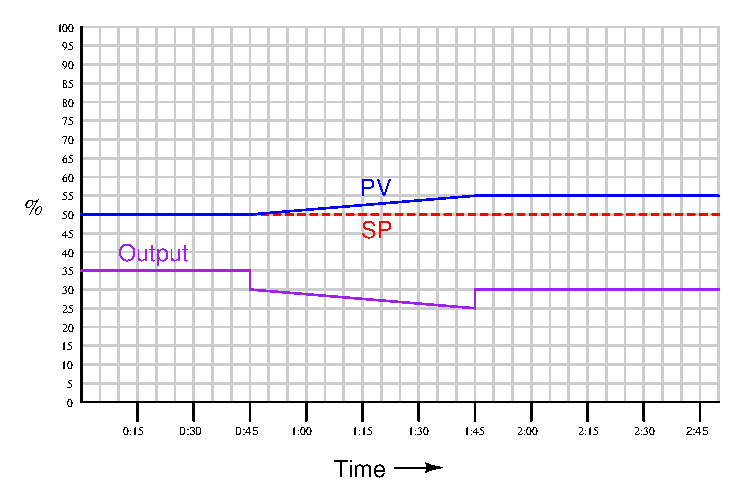
\includegraphics[width=15.5cm]{i01543x01.eps}$$

Tidsskalaen på diagrammet er minutter:sekunder.

\underbar{file i01543}
%(END_QUESTION)





%(BEGIN_ANSWER)

Regulatorvirkning = {\it revers}

\vskip 10pt

$K_p$ = 1

\vskip 10pt

$\tau_d$ = 1 minutt = 60 sekunder

\vskip 10pt

$$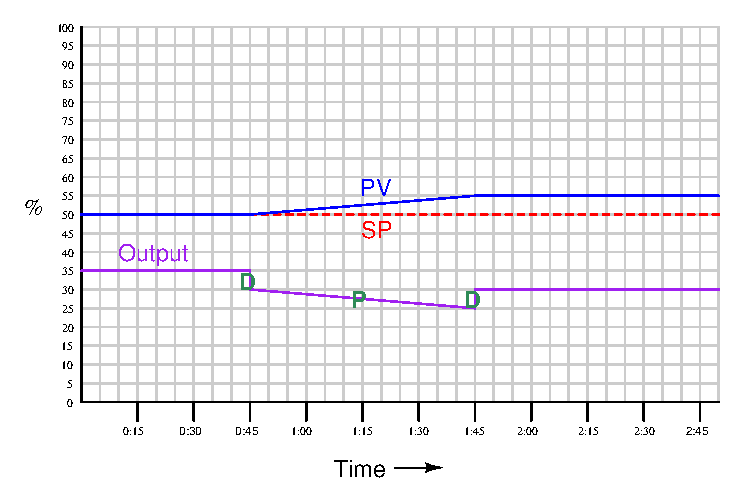
\includegraphics[width=15.5cm]{i01543x02.eps}$$

%(END_ANSWER)





%(BEGIN_NOTES)



%INDEX% Control, proportional + derivative: graphing controller response

%(END_NOTES)

